\documentclass{ethz_report}
\usepackage{listings}
\usepackage{color}
\usepackage{caption}
\usepackage{subcaption}


\definecolor{codegreen}{rgb}{0,0.6,0}
\definecolor{codegray}{rgb}{0.5,0.5,0.5}
\definecolor{codepurple}{rgb}{0.58,0,0.82}
\definecolor{backcolour}{rgb}{1,1,1}

\lstdefinestyle{mystyle}{
    backgroundcolor=\color{backcolour},
    commentstyle=\color{codegreen},
    keywordstyle=\color{magenta},
    numberstyle=\tiny\color{codegray},
    stringstyle=\color{codepurple},
    basicstyle=\ttfamily,
    breakatwhitespace=false,
    breaklines=true,
    captionpos=b,
    keepspaces=true,
    numbers=left,
    numbersep=5pt,
    showspaces=false,
    showstringspaces=false,
    showtabs=false,
    tabsize=4,
    frame=lines
}
\lstset{style=mystyle}

\title{Exercise 1 - Features}
\subject{Computer Vision}
\author{Alberto Montes}
\email{malberto@student.ethz.ch}
\date{\today}

\begin{document}
\maketitle

\section{Harris Corner Detector}

The implementation of the Harris Corner Detector starts with the computation of the image's
gradient. This step presented a problem as it was computed using a convolution, because corner
detection appeared at the margins of the image. This was solved padding symmetrically before
convolving as is shown in Listing~\ref{lst:gradient}

\lstinputlisting[language=MATLAB, caption=extractHarrisCorner.m, firstline=12, lastline=17, label={lst:gradient}]{../code/extractHarrisCorner.m}

Then each component of the Harris matrix was computed with this image gradient and a gaussian filter
to finally compute the Harris response mesure as:

\begin{equation}
    K = \frac{det(H)}{trace(H)} = \frac{I_x^2 \cdot I_y^2 - (I_x I_y)^2}{I_x^2 + I_y^2}
\end{equation}

Once the Harris response mesure has been computed, a Non-Maximum-Suppression operation must be
performed in order to obtain corners too close each one to the others. This can be easily see on the
following figure where the threshold was set to $3 \cdot 10^{-4}$ and it compares the use or not
of the Non-Maximum-Suppression operation.

\begin{figure}[H]
\centering
\begin{subfigure}[b]{.5\textwidth}
  \centering
  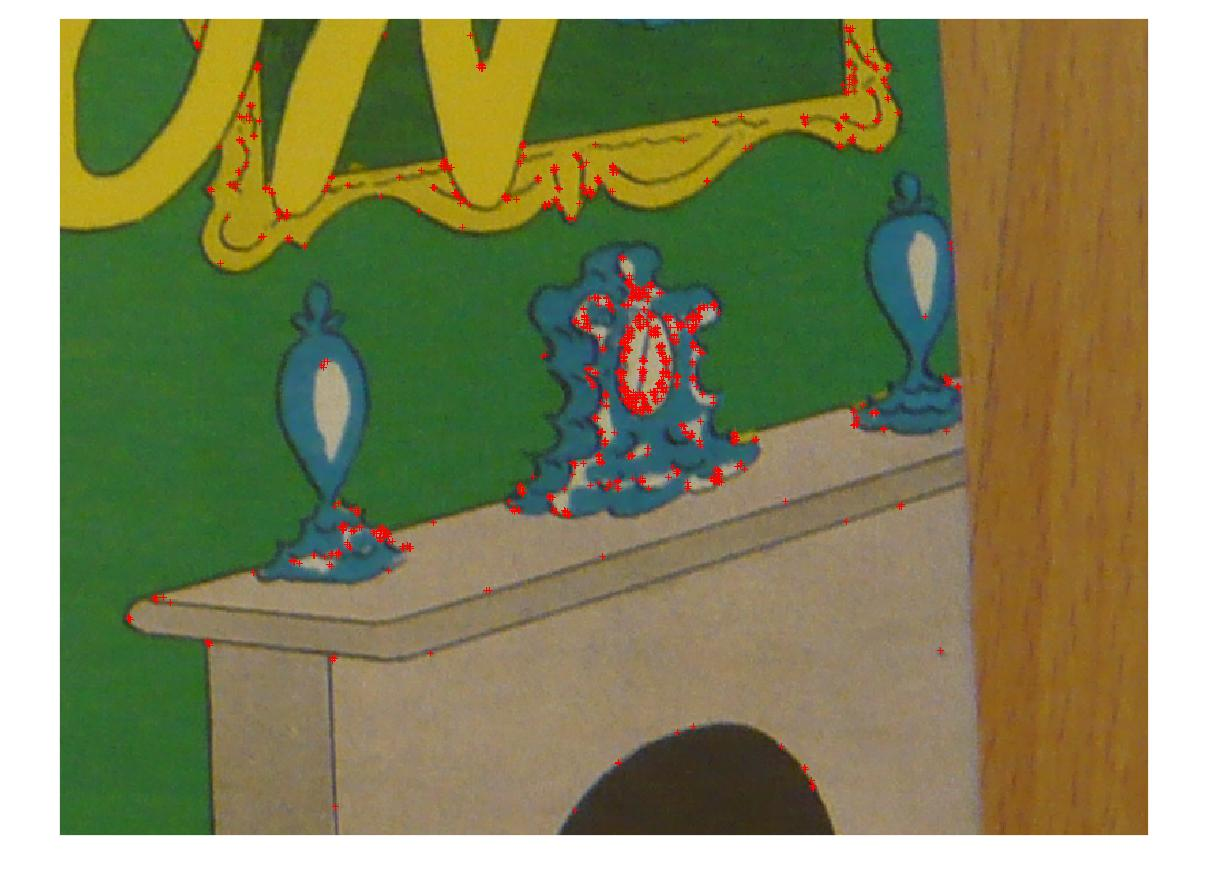
\includegraphics[width=1\linewidth]{images/harris_nms_before}
  \caption{Before applying Non-Maximal-Suppression}
\end{subfigure}%
\begin{subfigure}[b]{.5\textwidth}
  \centering
  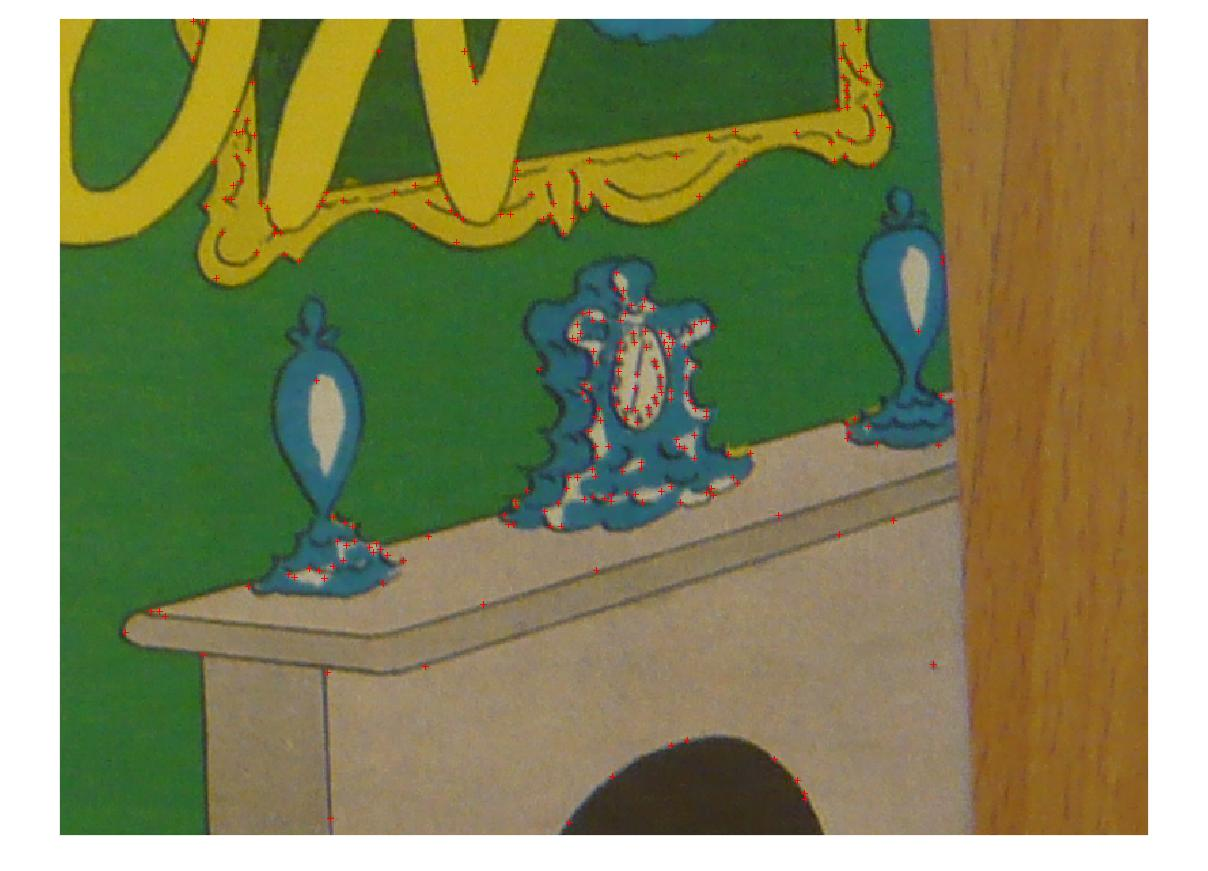
\includegraphics[width=1\linewidth]{images/harris_nms_after}
  \caption{After applying Non-Maximal-Suppression}
\end{subfigure}
\end{figure}

Finally the global images applying the Harris Corner Detector with a Non-Maximum-Suppression of 3
pixels of radius are displayed on Figure~\ref{img:corners}

\begin{figure}[H]
\centering
\begin{subfigure}[b]{.5\textwidth}
  \centering
  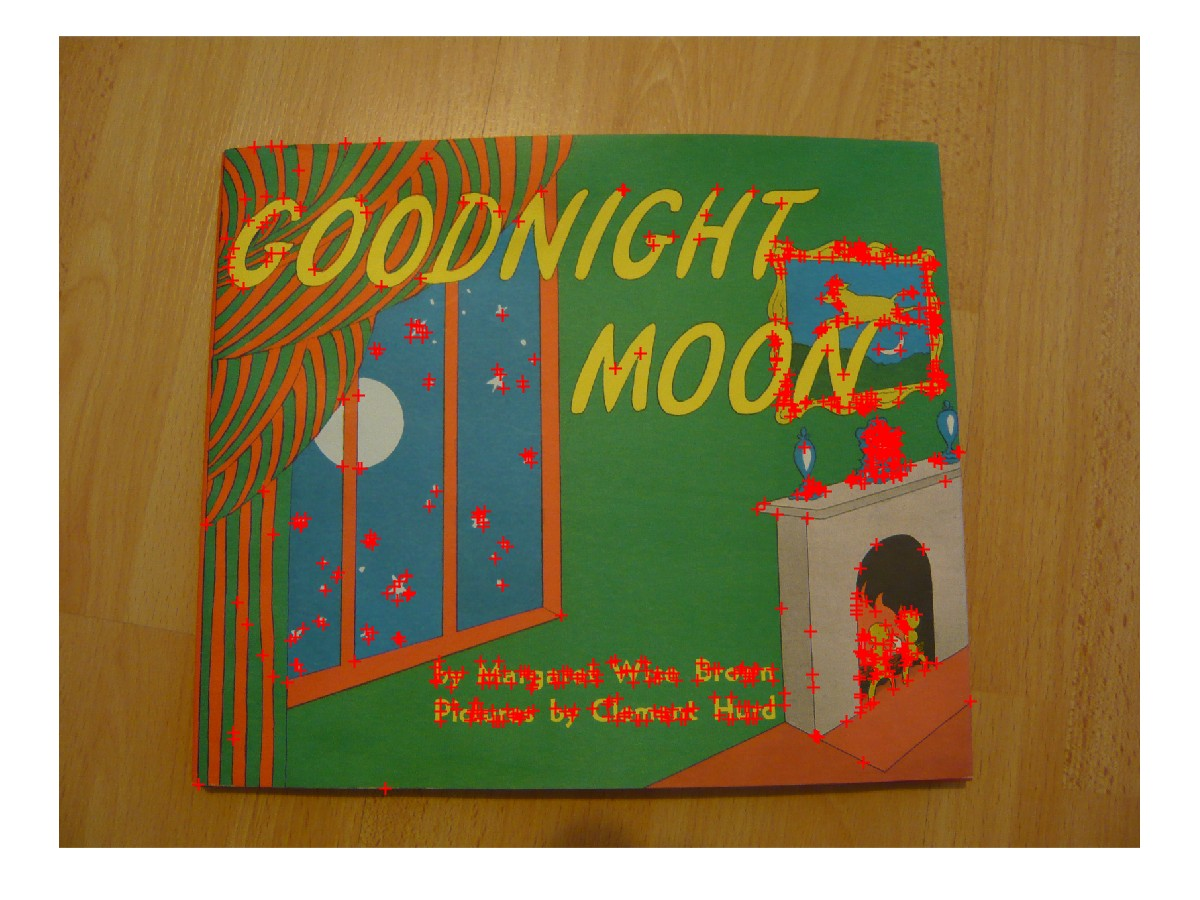
\includegraphics[width=1\linewidth]{images/corners1}
\end{subfigure}%
\begin{subfigure}[b]{.5\textwidth}
  \centering
  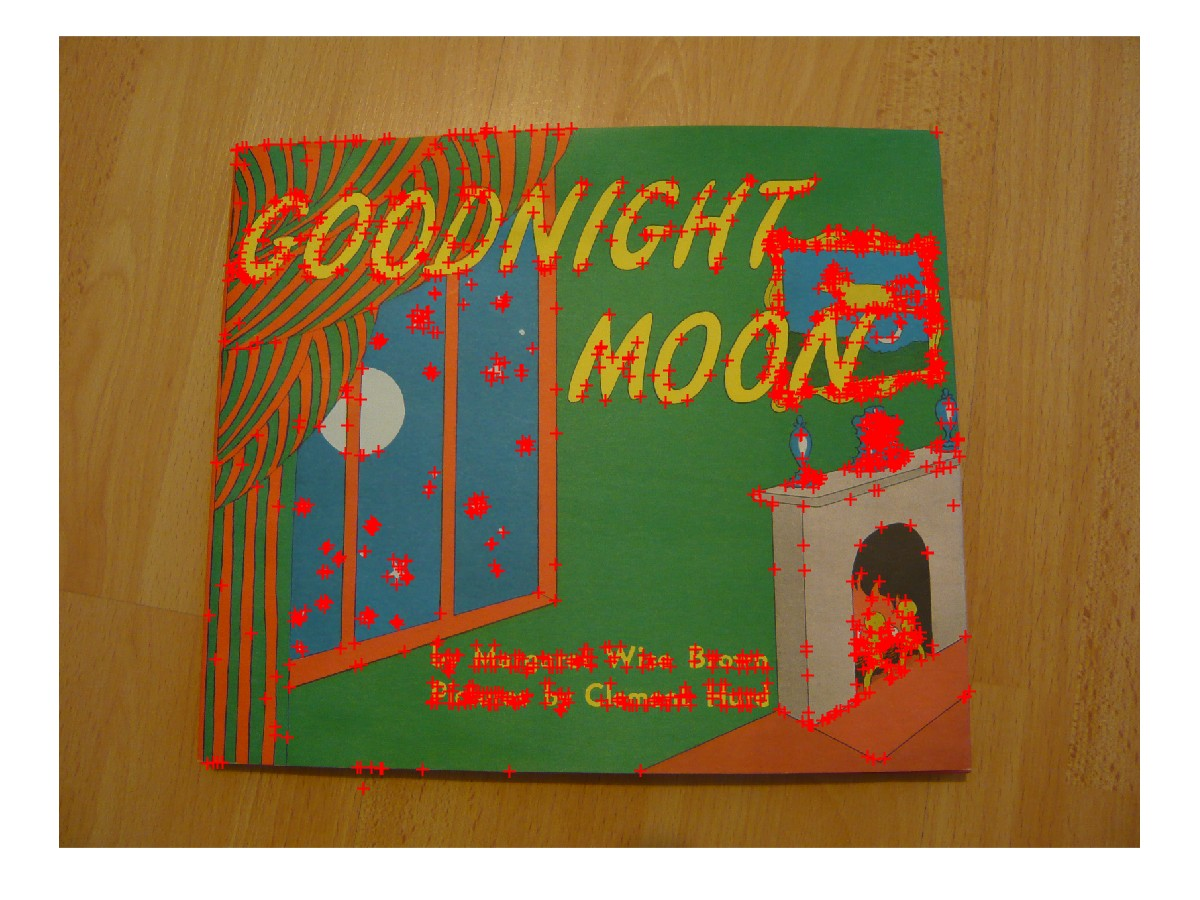
\includegraphics[width=1\linewidth]{images/corners2}
\end{subfigure}
\caption{Corners detected with the implementation of the Harris Corner Detector}
\label{img:corners}
\end{figure}

\section{Feature Matching}

After computing the corners, the SSD matching has been implemented. This did not present any major
issue except the threshold to set. Finally, this threshold was set to $0.8$ to get the maximum of
good matching and not so many wrong ones. In the Figure~\ref{img:matching} can be seen the matching
done using the Harris features extracted previously.

\begin{figure}[H]
\centering
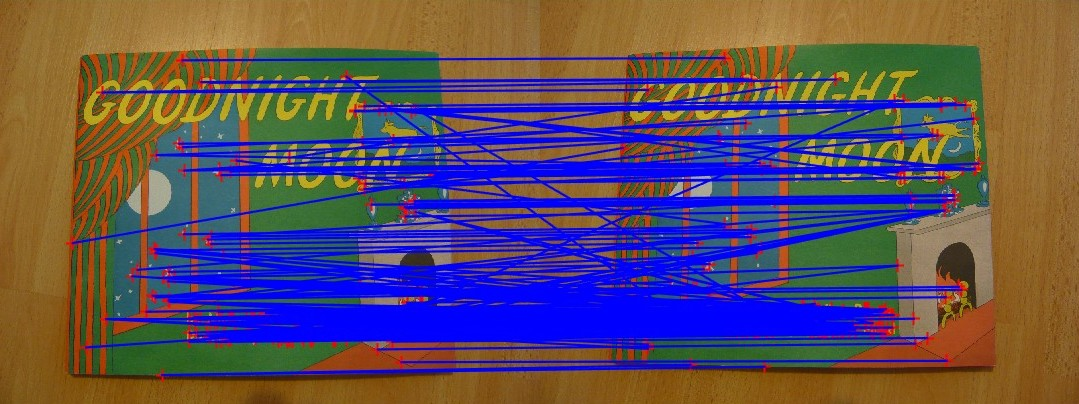
\includegraphics[width=1\linewidth]{images/matching_harris}
\caption{Matching of the Harris Corner features using the SSD.}
\label{img:matching}
\end{figure}

\section{SIFT features}

Using the library VLfeat provided, it has been possible to extract the SIFT features and compare
the results with the Harris features computed with my implementation. In the following figure it is
shown the Harris corner features and the SIFT features for the same image. The SIFT features was so
large that it is shown only 500 selected randomly from the ones provided by the VLfeat implementation.

\begin{figure}[H]
\centering
\begin{subfigure}[b]{.5\textwidth}
  \centering
  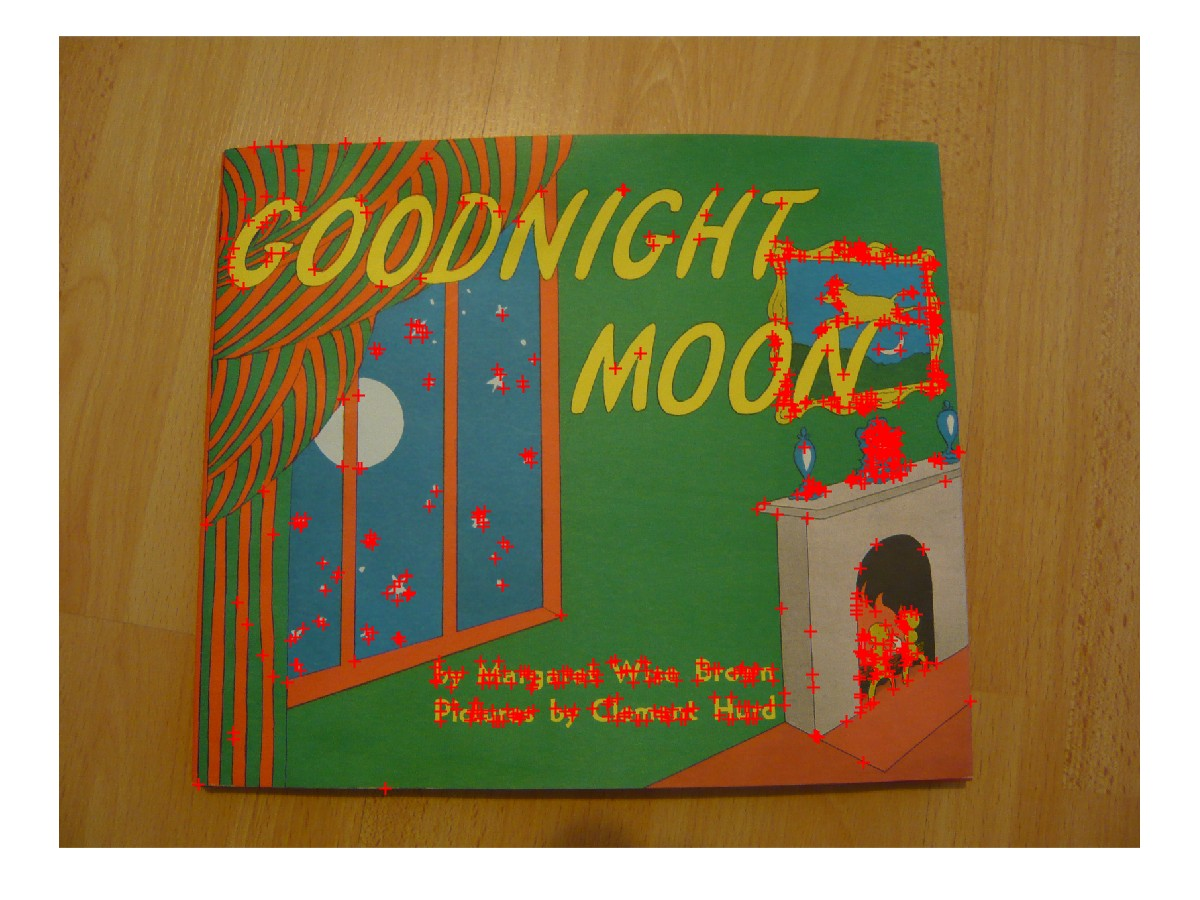
\includegraphics[width=1\linewidth]{images/corners1}
  \caption{Harris Corner Features}
\end{subfigure}%
\begin{subfigure}[b]{.5\textwidth}
  \centering
  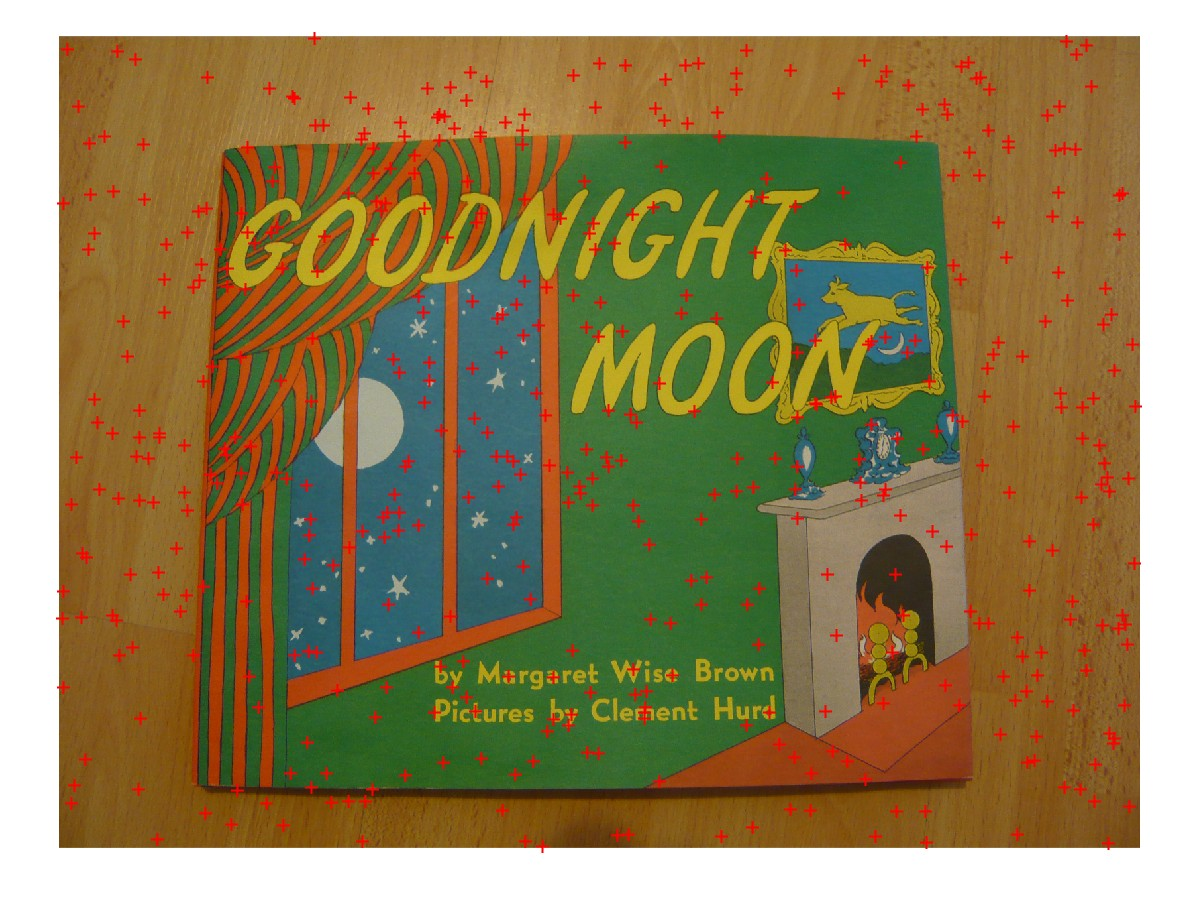
\includegraphics[width=1\linewidth]{images/sift1}
  \caption{SIFT Features}
\end{subfigure}
\caption{Comparison between Harris and SIFT features.}
\end{figure}
\label{img:comparison_features}

As can be seen on Figure~\ref{img:comparison_features}, the Harris Corner detector find the corners
of the image and activate its detections on edges of the image. At the same time, the SIFT features
seem to be more distributed along the images, activating even on flat textures, which gives more
information at the time to do the matching.

\begin{figure}[H]
\centering
\begin{subfigure}[b]{\textwidth}
  \centering
  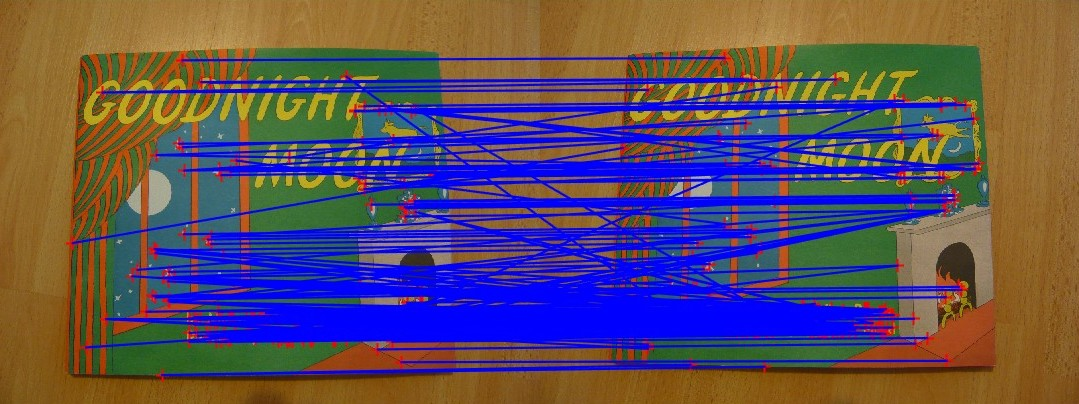
\includegraphics[width=1\linewidth]{images/matching_harris}
  \caption{Harris Corner Features Matching}
\end{subfigure}
\begin{subfigure}[b]{\textwidth}
  \centering
  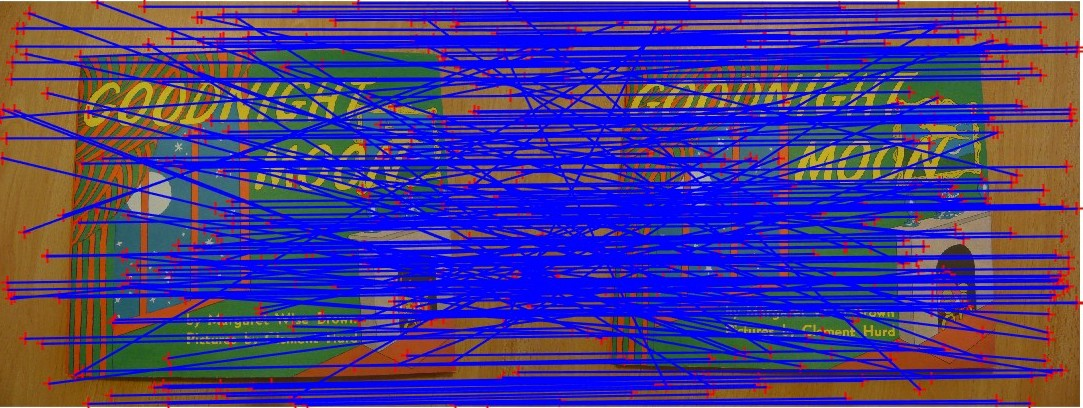
\includegraphics[width=1\linewidth]{images/matching_sift}
  \caption{SIFT Features Matching}
\end{subfigure}
\caption{Comparison between Harris and SIFT features matching.}
\label{img:comparison_features_matching}
\end{figure}

In Figure~\ref{img:comparison_features_matching} can be seen how there is more matchings using the
SIFT features as there are more of them even on more plain textures, where the Harris features
matches the ones corresponding to more sharp textures as corners and edges.

\end{document}
